\documentclass[12 pt]{article}
\usepackage[utf8]{inputenc}
\usepackage{graphicx}
\usepackage{amsmath}
\usepackage{amssymb}
\usepackage{multirow}
\usepackage{caption}
\usepackage{subcaption}
\usepackage{hyperref}
\usepackage{pgf}
\usepackage{pgfpages}
\usepackage{textcomp}
\usepackage{lscape}
\usepackage{geometry}
\usepackage{pdflscape} 
\usepackage{placeins}
\usepackage{url}
\usepackage{natbib}
%\usepackage[a4paper,margin=1in]{geometry}

\pgfpagesdeclarelayout{boxed}
{
  \edef\pgfpageoptionborder{0pt}
}
{
  \pgfpagesphysicalpageoptions
  {%
    logical pages=1,%
  }
  \pgfpageslogicalpageoptions{1}
  {
    border code=\pgfsetlinewidth{2pt}\pgfstroke,%
    border shrink=\pgfpageoptionborder,%
    resized width=.95\pgfphysicalwidth,%
    resized height=.95\pgfphysicalheight,%
    center=\pgfpoint{.5\pgfphysicalwidth}{.5\pgfphysicalheight}%
  }%
}

\pgfpagesuselayout{boxed}

\title{Assignment 1}
\author{Abhijeet Mangela}
\date{November 2022}

\title{Assignment 1}
\author{Abhijeet Mangela}
\date{\today}

\begin{document}
\begin{titlepage}
\begin{center}

\textbf{\huge Design project report Group 7 \\ \vspace{0.4 cm} Week 2} \\

\vspace{2 cm}

\centering

\includegraphics[width=0.5\textwidth]{IIT_Madras_Logo.svg.png}
\label{fig:my_label}

\vspace{1cm}

\textbf{Abhijeet Mangela AE21B040 \\ Navin Yadav AE23M803 \\ Balamurugan S AE23M009 \\ Samarth R Krishna AE23M032 \\ Senthil B AE23M035 \\ Rajendran Anandhu Nair AE23M027 }

\vspace{0.5cm}

\footnotesize Department of Aerospace Engineering \\
IIT Madras \\
India

\normalsize

\end{center}
\end{titlepage}


\newpage

\tableofcontents

\newpage

\section{Introduction}

\subsection{Objective}
The primary objective of this design project is to design and fly a fixed wing UAV that can survey wildlife and monitor plastic free zones/environment in amusement parks, zoos and wildlife sanctuaries.


\subsection{Abstract}
Air quality is an essential measure of the quality of life of any living being. A decrease in air quality is easily linked with a reduction in the life expectancy of various plants and animals.

As a result, we are focused on working on a drone that will give us an insight into the air quality of a region. 

We often have to measure air quality within a forest or a region where it is hard to go physically. As a result, we have to place expensive monitoring sensors at various challenging-to-reach locations. 

When some maintenance issues arise in these sensors, we again have to send teams to repair the equipment.

These complications can be reduced by using a fixed-wing UAV instead of ground sensors because the UAV is a moving object that can cover a larger area than a UAV sensor alone. Also, if some maintenance problem arises, it can be fixed when the UAV lands.

The UAV will also carry out visual surveillance of the land it is flying. A direct flight will provide a better and more frequent information intake than satellite imagery.

\subsection{Mission Profile and requirements}

\subsubsection{Mission Requirement}
%Our objective is to detect the gases present near the aeroplane. It should detect elements including PM2.5, PM10, O3, NO2, SO2, CO, VOCs, H2S, NH3, HCl, CxHy, H2 and more.
In the event of a crowd gathering, ensuring the cleanliness of a natural environment conducive to the dwelling of fauna is challenging. To overcome this problem steadfastly without affecting the crowd's morale, instead of acting as an entertainment element in satisfying the objective above, UAVs are identified as the best choices amidst these situations. 


The UAV will be equipped with air quality sensors and cameras to understand the terrain better. Thus, knowledge about plastics and unpleasant atmospheres will help develop a quick action plan for maintaining the flora and fauna from foreign hazards.

\subsubsection{Aircraft Characteristics}
\begin{table}[h]
\centering
\resizebox{0.6\textwidth}{!}{%
\begin{tabular}{|c|c|}
\hline
\textbf{Estimated MTOW}            & 8 – 10 kg                \\ \hline
\textbf{Maximum Payload Weight}    & 1 – 1.5 kg               \\ \hline
\textbf{Estimated Endurance}       & 30 minutes               \\ \hline
\textbf{Mission ceiling}           & 0 - 250 m                \\ \hline
\textbf{Desired Operational Speed} & 27 m/s                   \\ \hline
\textbf{Transmitter Range}         & 4 km                     \\ \hline
\end{tabular}%
}
\end{table}

\subsubsection{Payload measure}
The payload of UAVs consists of a camera and a sensor module used to measure air quality. The camera will be a Hontral B0BMV12VYJ HD Camera weighing 492 g. The sensor module comprises Arduino MKR Proto Large Shield TSX00002, weighing about 200 g and sensors such as MQ-7 CO Carbon Monoxide, MG811 Air Carbon Dioxide, etc., weighing about 320 g.

\subsection{Mission Profile}

\begin{figure}[h]
    \centering
    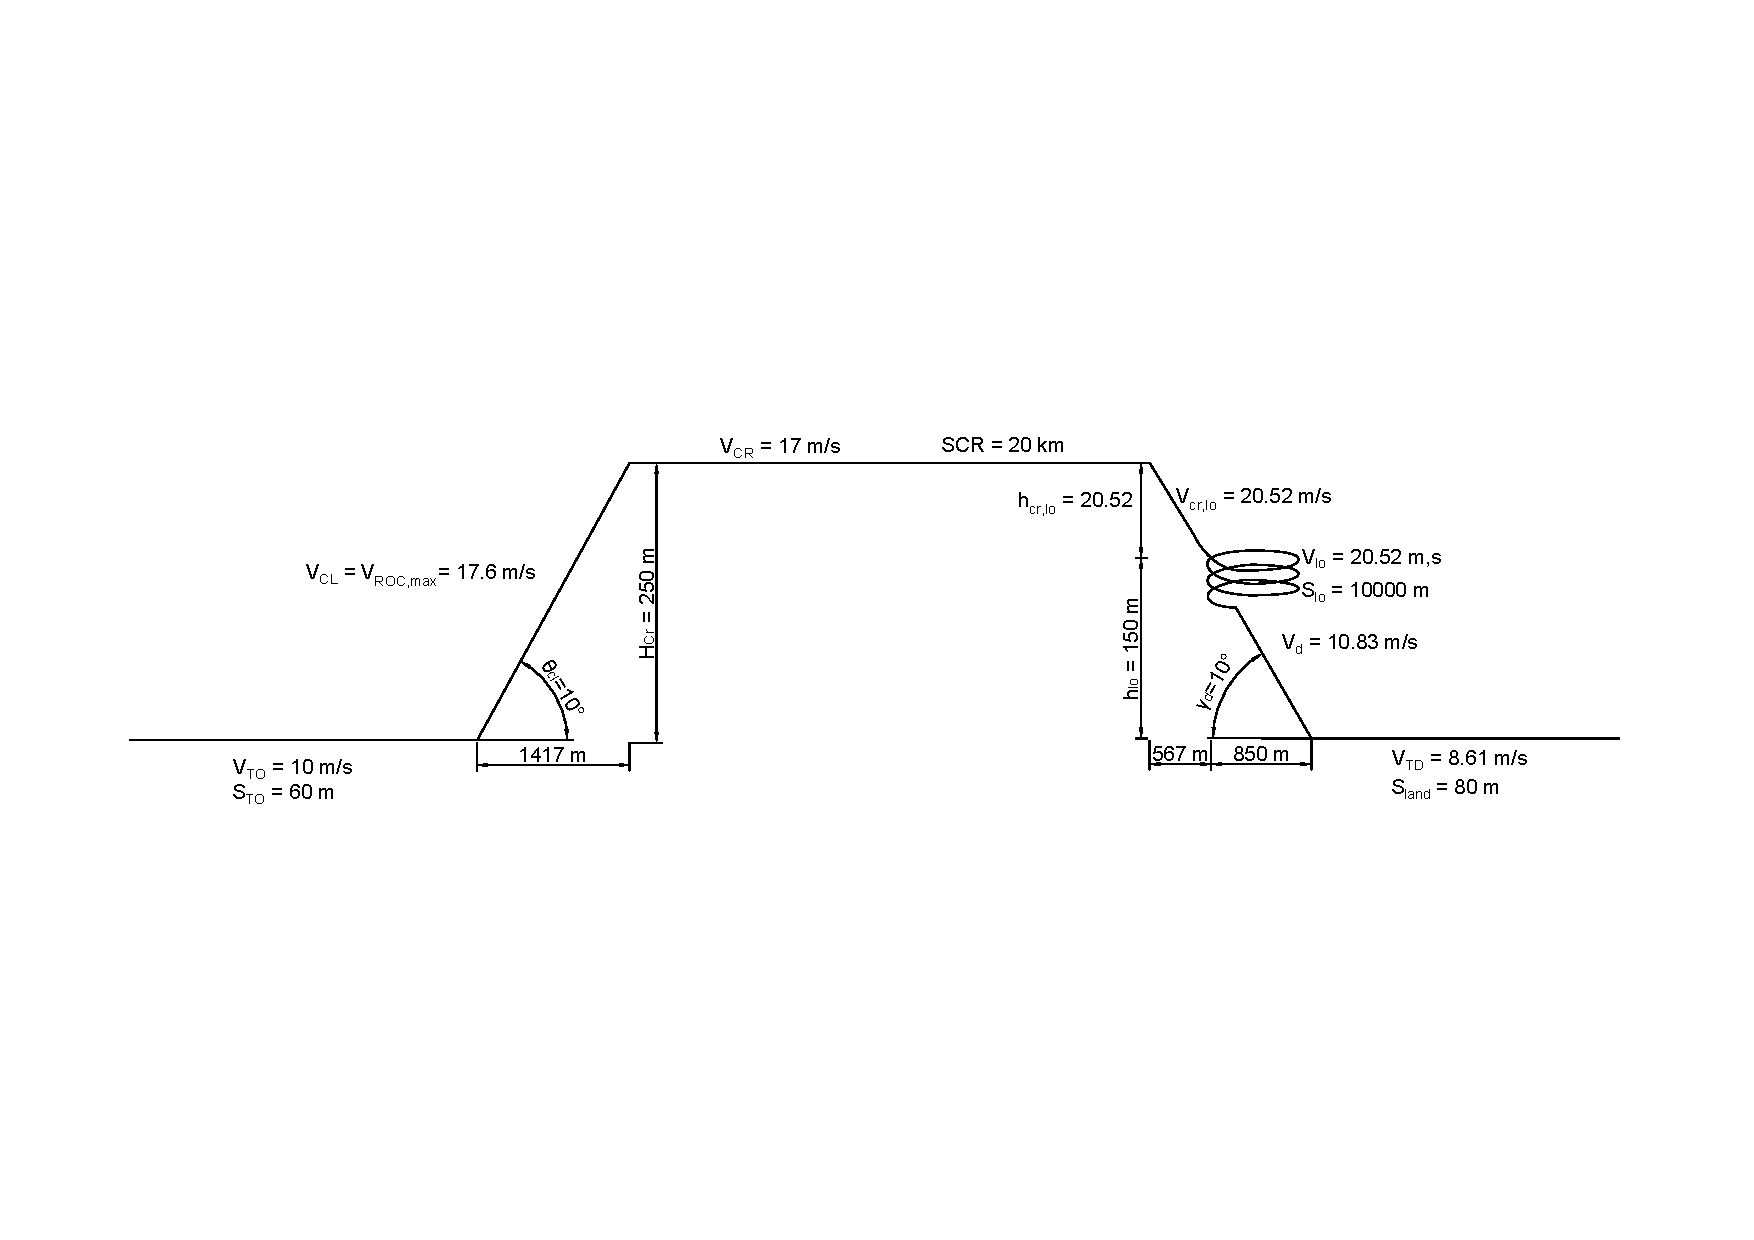
\includegraphics[width = \linewidth]{Drawing1-Model_final.pdf}
    \caption{Caption}
    \label{fig:enter-label}
\end{figure}


\subsubsection{Ground run}
The take-off ground run distance is approximately 60 metres and estimated take-off velocity is 10 m/s. \cite{EgglestonUnknownTitle2015}

$$ (V_{TO})_{_{Bricans \: Td100}} = 19 \: m/s$$
$$ (W_{TO})_{_{Bricans \: Td100}} = 22.67 \: kg$$

Since $ V_{TO} \: \alpha \: \sqrt{W_{TO}} $ for given $C_L$ , S (applicable for initial estimate)

$$ (V_{TO})_{_{des}} = (V_{TO})_{_{Bricans \: Td100}} \times \sqrt{\frac{(W_{TO})_{_{des}}}{(W_{TO})_{_{Bricans \: TD \: 100}}}} $$

$$ = 19 \times \sqrt{\frac{5.6 \times 9.81}{22.67 \times 9.81}} = 9.94 \: m/s \approx 10 \: m/s $$

\subsubsection{Climb \cite{1000_questions} }
The UAV will climb at an estimated velocity of 17.6 m/s to operating altitude of 250 m AMSL. The rate of climb is about 3.06 m/s. Time spent here 81.7 s

Calculation :- 
$$ (V_{TO})_{_{des}} = 10 \: m/s \Rightarrow (V_{stall})_{_{des}} = \frac{(V_{TO})_{_{des}}}{1.2} = 8.33 \: m/s $$
$$ (V_{md})_{_{des}} = 1.6 \times V_{stall} = 13.33 \: m/s $$
$$ (V_{ROC})_{_{max}} = 1.32 \times V_{md} = 17.6 \: m/s $$

\subsubsection{Cruise \cite{alhajjaji2017design}}
The UAV will perform aerial surveillance and environmentally monitor for areas of plastics and solid waste with an estimated cruise speed of 17 m/s for 20 km range. Time spent here is 1176 s.

\subsubsection{Descent to Mission Height}
The UAV will descend to 150 m altitude AMSL to study air quality at a sinking speed of 20.52 m/s for 5 km range. Time spent here is 28 s.

Calculation: - 
$$ (V_{cr,lo})_{_{design}} = 0.76 \times (V_{cr})_{_{des}} \;  (initial \: estimate) $$
$$ = 20.52 \: m/s $$

\subsubsection{Descent to land \cite{Anderson1}}
The UAV will descend at an estimated velocity of 10.13 m/s. To close ground proximity, the UAV is gradually decelerated to an estimated touchdown velocity of 8.61 m/s. Time spent here is 80 s.
Calculation: - 
$$(V_des)_{_{design}} = (V_{mg})_{_{design}} = (V_{mg})_{_{design}} \times 0.76 = 10.13 \: m/s $$

\subsubsection{Landing run}
The landing ground run distance is approximately 80 metres and estimated touchdown velocity is 8.61 m/s.

Calculation: - 
$$ (V_{TD})_{_{design}} = 0.85 \times (V_{des})_{_{design}} = 8.61 \: m/s  $$
$$ \text{Vertical component of } (V_{TD})_{_{design}} = 8.61 \times \sin{10^{\circ}} $$
$$ = 1.495 \: m/s \leq 4 \: m/s \; \text{(For smooth landing)} $$



\subsection{Data collection}

The data of all the parameters:-
% Please add the following required packages to your document preamble:
% \usepackage{graphicx}
\begin{table}[h]
\centering
\resizebox{\textwidth}{!}{%
\begin{tabular}{|c|c|c|c|c|c|c|c|}
\hline
SI no &
  UAV Name &
  \begin{tabular}[c]{@{}c@{}}MTOW \\ Kg\end{tabular} &
  \begin{tabular}[c]{@{}c@{}}Empty Weight\\ kg\end{tabular} &
  \begin{tabular}[c]{@{}c@{}}Battery Weight\\ kg\end{tabular} &
  \begin{tabular}[c]{@{}c@{}}Payload Weight\\ kg\end{tabular} &
  \begin{tabular}[c]{@{}c@{}}Range \\ km\end{tabular} &
  \begin{tabular}[c]{@{}c@{}}Endurance\\ min\end{tabular} \\ \hline
1 & Wingtraone   \cite{Wingtra}             & 4.5 & 2.387 & 0.604       & 1.509 &     & 59  \\ \hline
2 & Albatross    \cite{Albatross}             & 10  & 3.5   & 2.4         & 4.1   & 250 & 240 \\ \hline
3 & Azimut   2    \cite{Azimut}            & 9   & 2.5   & 2.8         & 3.7   &     &     \\ \hline
4 & Dragonfly   Tango 2  \cite{Dragonfly}      & 5   & 3     & 0.595+0.595 & 1.5   & 5   & 120 \\ \hline
5 & Nostromo   Defensa Cabure \cite{Nostromo} & 5   & 3.4   & 0.604       & 1     & 15  & 1.5 \\ \hline
6 & SPY   LITE    \cite{Bluebird}            & 9.5 & 4.5   & 1.5         & 1.35  & 80  & 240 \\ \hline
7 & Skylark I-LEX   \cite{Skylark}          & 7.5 & 5.5   & 0.8         & 1.2   & 40  & 180 \\ \hline
\end{tabular}%
}
\caption{Data part one}
\label{tab:my-table}
\end{table}

% Please add the following required packages to your document preamble:
% \usepackage{graphicx}
\begin{table}[h]
\centering
\resizebox{\textwidth}{!}{%
\begin{tabular}{|c|c|c|c|c|c|c|c|c|c|}
\hline
SI no &
  UAV Name &
  \begin{tabular}[c]{@{}c@{}}Service Ceiling\\ m\end{tabular} &
  \begin{tabular}[c]{@{}c@{}}Maximum Ceiling\\ m\end{tabular} &
  \begin{tabular}[c]{@{}c@{}}Cruise speed\\ km/hr\end{tabular} &
  \begin{tabular}[c]{@{}c@{}}Max Speed\\ km/hr\end{tabular} &
  \begin{tabular}[c]{@{}c@{}}Longitudinal Length\\ cm\end{tabular} &
  \begin{tabular}[c]{@{}c@{}}Wing Span\\ cm\end{tabular} &
  AR &
  L/D \\ \hline
1 & Wingtraone                & 120  & 2500   to 5000 & 35.8 &     &     & 125 & 1.838 &                \\ \hline
2 & Albatross                 &      &                & 68   & 129 &     & 300 &       & 28:1   to 30:1 \\ \hline
3 & Azimut   2                &      &                &      &     &     &     &       &                \\ \hline
4 & Dragonfly   Tango 2       &      &                & 43.2 & 100 &     &     &       &                \\ \hline
5 & Nostromo   Defensa Cabure & 4000 &                & 70   & 105 &     &     &       &                \\ \hline
6 & SPY   LITE                &      &                &      & 120 & 135 & 275 &       &                \\ \hline
7 & Skylark I-LEX             & 4572 &                & 37   & 74  & 220 & 300 &       &                \\ \hline
\end{tabular}%
}
\caption{Additional data}
\label{tab:my-table}
\end{table}

\begin{figure}[h!]
    \centering
    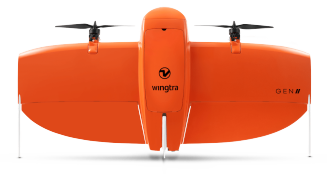
\includegraphics[width=0.7\linewidth]{Aircraft pics/WingtraOne.png}
    \caption{Wingtraone}
    \label{fig:enter-label}
\end{figure}

\begin{figure}[h!]
    \centering
    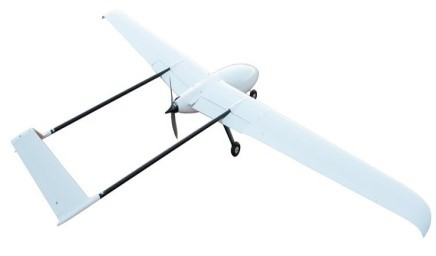
\includegraphics[width=0.7\linewidth]{Aircraft pics/Albatross.jpg}
    \caption{Albatross}
    \label{fig:enter-label}
\end{figure}

\vspace{\fill}

\newpage

\begin{figure}[h!]
    \centering
    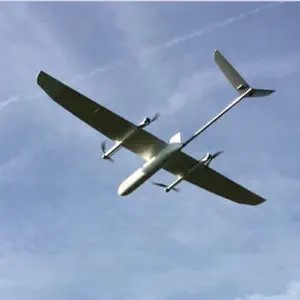
\includegraphics[width=0.35\linewidth]{Aircraft pics/Azimut.jpg}
    \caption{Azimut 2}
    \label{fig:enter-label}
\end{figure}

\begin{figure}[h!]
    \centering
    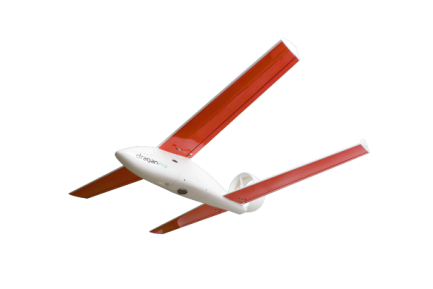
\includegraphics[width=0.55\linewidth]{Aircraft pics/Dragonfly.png}
    \caption{Dragonfly Tango 2}
    \label{fig:enter-label}
\end{figure}

\begin{figure}[h!]
    \centering
    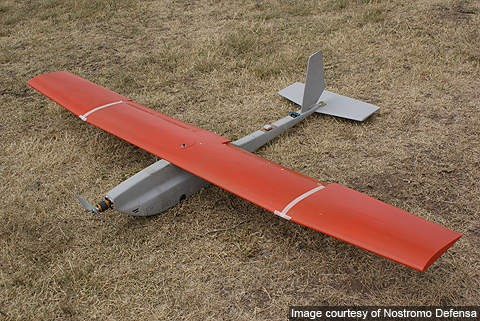
\includegraphics[width=0.45\linewidth]{Aircraft pics/Nostroma.jpg}
    \caption{Nostroma Defensa Cadambra}
    \label{fig:enter-label}
\end{figure}

\begin{figure}[h]
    \centering
    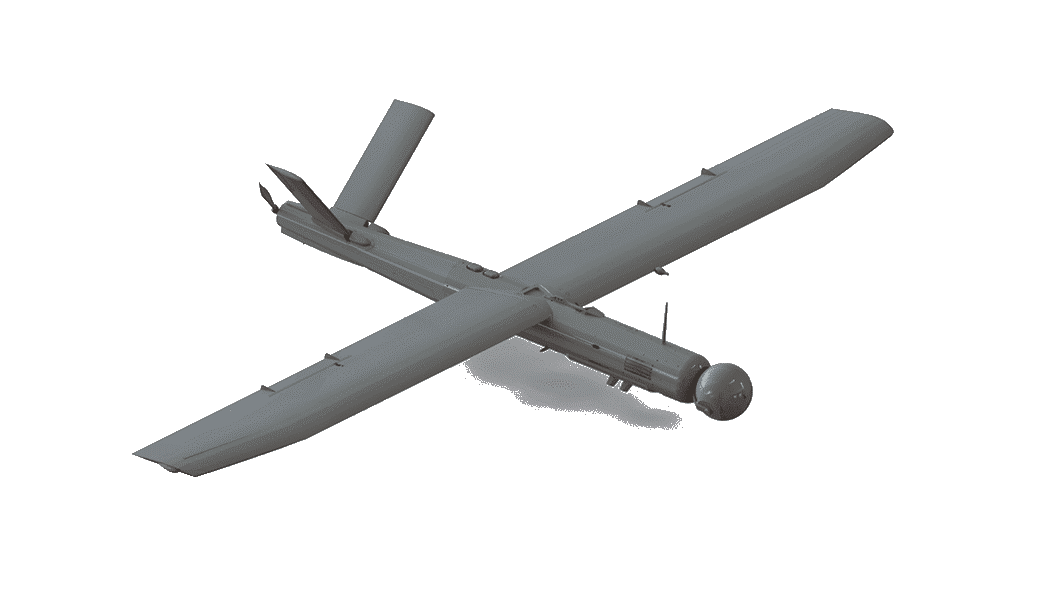
\includegraphics[width=0.5\linewidth]{Aircraft pics/spylite.png}
    \caption{Spylite}
    \label{fig:enter-label}
\end{figure}

\begin{figure}[h]
    \centering
    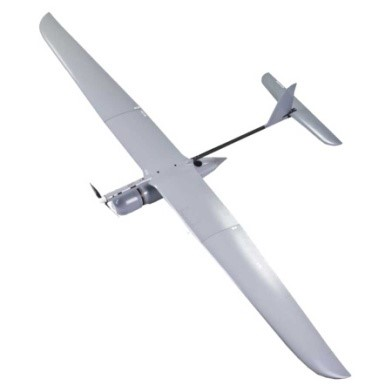
\includegraphics[width=0.3\linewidth]{Aircraft pics/Skylark.jpg}
    \caption{Skylark}
    \label{fig:enter-label}
\end{figure}

\newpage

%\Floatbarrier
%\vspace{\vfill}

\section{Preliminary Weight estimation}

Weight estimation is divided into various sections
\subsection{Payload weight estimation}
Rough estimate for payload
\begin{table}[h]
\centering
\resizebox{0.6\textwidth}{!}{%
\begin{tabular}{|c|c|}
\hline
Purpose                            & Weight \\ \hline
Camera                             & 492 g  \\ \hline
Sensor module                      & 520 g  \\ \hline
Bulk Tolerance (Wiring, Actuation) & 388 g  \\ \hline
Total Payload Estimate             & 1400 g \\ \hline
\end{tabular}%
}
\end{table}

\hfill


\subsection{Empty weight estimation}
The empty weight ratio can be estimated from the previous data. We have to fit the data in the curve of $y = A x^c$ with A and C as variables.

In our Data A is 1.7086 and C is -0.67155.

\begin{figure}[h]
    \centering
    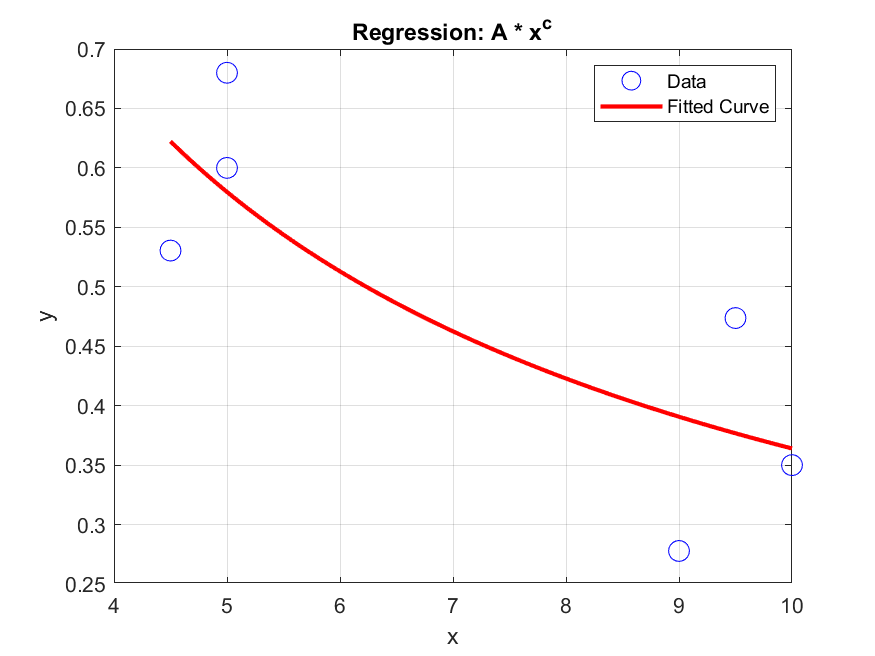
\includegraphics[width = \linewidth]{Regression.png}
    \caption{Empty weight estimation}
    \label{fig:enter-label}
\end{figure}

\newpage

\subsection{Battery weight estimation}

Battery is an important criteria for design of any drone. We should optimise the battery weight in accordance with the Mission profile we have. That way we will not be carrying unnecessary dead weight with us.

For calculating Battery weight estimation we have to first find out the total energy required for each Major phase on flight.

\subsubsection{Cruise}
Now for a level flight,
$$ L = D \; \; , \; \; T = D$$

$$ W = \frac{1}{2} \rho V^2 S C_L $$
$$ C_L = \frac{W}{\frac{1}{2} \rho V^2 S}$$
So,
$$ C_D = C_{D_0} + \frac{C_L^2}{\pi 2 AR} $$
Now 
$$ P = TV = DV $$

So, 
$$ P_R = \frac{1}{2}\rho V^3 S C_{D_o} + \frac{2 W^2}{ (\rho V S) \pi e AR} $$

$$P_R = f(W,\rho,V,C_{D_o},S,e,AR)$$

Taking approximations and inputting mission profile conditions

$$ P_R = f(W) $$

We will consider Loitor phase as cruise too.

\subsubsection{Climb }
Power required for climb is given by 
$$ P = W \times R.O.C + P_R $$

\subsubsection{Descent}
Power required for descent is 
$$ P = P_R - W \times Rate\: of\: descent$$
We need to take care that the power does not go negative here or make it zero while estimating energy.

\subsection{Take off and Landing}
The Segments of take off and landing do not take that much time in general. Also it is harder to get an accurate estimate of the energy spent in takeoff and landing due to the carrying power needs. So we will take an 

\subsubsection{Battery weight}

We can calculate the energy by multiplying power required times the amount of time spent in that phase. From energy we can get battery weight by dividing it with energy density. 

For lithium polymer batteries, the energy density is around 273600.

\section{Total weight estimation}

The total weight is given as :- 
$$ W_0 = W_{pl} + W_{e} + W_{f} $$
Where,
\begin{itemize}
    \item[-] $W_0$ is the total design weight.
    \item [-] $W_{pl}$ is the payload weight.
    \item [-] $W_{e}$ is the empty weight.
    \item [-] $W_{f}$ is the fuel weight (Battery in our case).
\end{itemize}

It can be transformed into :- 
$$W_{0} = \frac{W_{pl}}{1 - \frac{W_{e}}{W_{0}} - \frac{W_{f}}{W_0}}$$

If we have an initial approximation, we can run an iteration algorithm to find out design weight when we keep empty weight ratio as a variable.

Generally we take an initial estimate to be 4 times the payload weight. Taking the correct initial weight is very important or the code may blow up.

In our case the design weight came out to be 5.27 kg.

\begin{figure}
    \centering
    \includegraphics[width=0.75\linewidth]{Codes/}
    \caption{Enter Caption}
    \label{fig:enter-label}
\end{figure}

\vfill

\newpage

\appendix

\newpage

\section{References}

\bibliographystyle{IEEEtran}
\bibliography{References}

\newpage

\section{Changes}

\subsection{Week 2}
\begin{enumerate}
    \item Data collection part was completely changed.
    \item The general design of pdf was changed.
    \item More data was added along with a table for better comparison.
    \item Battery performance was estimated.
    \item Weight was estimated.
    \item References were added.
    \item The Mission profile was updated.
    \item Details on mission profile were added.
\end{enumerate}

\subsection{Week 3}

\newpage

\section{Contributions}

\subsection{Week 2}

\subsubsection{Abhijeet Mangela AE21B040}
Wrote full Latek report, Drew the mission profile with Inkscape and Autocad, Empty weight Fraction estimation, Final weight estimation with Senthil

\subsubsection{Navin Yadav AE23M803}

Data Collection; Literature Survey

\subsubection{Balamurugan S AE23M009}

Data Collection; Literature Survey

\subsubsection{Samarth R Krishna AE23M032}

Data Collection; Literature Survey

\subsubsection{Senthil B AE23M035}

Detailed Mission Profile; Preliminary Weight Estimation (only iteration) ; Battery weight estimation.

\subsubsection{Rajendran Anandhu Nair AE23M027}

Data Collection; Literature Survey




\subsection{Week 3}

\subsubsection{Abhijeet Mangela AE21B040}


\subsubsection{Navin Yadav AE23M803}


\subssubection{Balamurugan S AE23M009}



\subsubsection{Samarth R Krishna AE23M032}



\subsubsection{Senthil B AE23M035}



\subsubsection{Rajendran Anandhu Nair AE23M027}



\section{Current estimates}

\end{document}
